\section{Background Subtraction and Person Isolation}
\label{background subtraction and person isolation}
In order to create a point cloud of a person, the tool kit must be able to isolate the person being scanned from the background environment. This is a well researched problem and is an issue for many applications in the computer vision field. Background subtraction is a commonly used class of techniques for segmenting out objects of interest in a scene for applications such as surveillance \cite{McIvor2000}. Even though many background subtraction algorithms have been proposed in the literature, the problem of identifying moving objects in complex environment is still far from being completely solved \cite{Cheung2007}.\\

There are many algorithms for isolating objects and relatively few, to no, algorithms specifically designed to isolate only a person. Therefore, research focused on generic isolation algorithms.\\

\subsection{General Approaches, Properties and Steps}
A common approach for isolating general objects is to perform background subtraction, which identifies moving objects from the portion of a video frame that differs significantly from a background model \cite{Cheung2007}.
This general approach allows the isolation of non humanoid objects such as cars, but is still worthy of note because any person isolation algorithm must shared some similarities with generic object isolation algorithms.\\

These similarities between the algorithms for object isolation and person isolation are that both must \cite{Cheung2007}:\begin{itemize}
  \item Be robust against changes in illumination
  \item Avoid detecting non-stationary background objects such as swinging leaves
  \item React quickly to changes
\end{itemize}

Approaches to object isolation vary from simple techniques such as frame differencing and adaptive median filtering, to more sophisticated probabilistic modelling techniques. 
While complicated techniques often produce superior performance, experiments \cite{Cheung2007} show that simple techniques such as adaptive median filtering can produce good results with much lower computational complexity.\\

In general, the four major steps in a background subtraction algorithm are preprocessing, background modelling, foreground detection, and data validation.
Preprocessing consists of a collection of simple image processing tasks that change the raw input video into a format that can be processed by subsequent steps and can involve noise reduction and frame size/rate reductions \cite{Cheung2007}\\.

Background modelling uses the new video frame to calculate and update a background model.
This background model provides a statistical description of the entire background scene and can be non-recursive or recursive. 
A non-recursive technique uses a sliding-window approach for background estimation. 
The technique stores a buffer of the previous $L$ video frames, and estimates the background image based on the temporal variation of each pixel within the buffer.
Non-recursive techniques are highly adaptive as they do not depend on the history beyond those frames stored in the buffer \cite{Cheung2007}, which may make the ideal for the tool kit.
On the other hand, the storage requirement can be significant if a large buffer
is needed to cope with slow-moving objects \cite{Cheung2007}, although that should not be a problem for the tool kit. Recursive techniques do not use a buffer but maintain a single background model based on each input frame. As a result, input frames from distant past could have an effect on the current background model \cite{Cheung2007} and hence may not be suitable for the tool kit.\\

Foreground detection then identifies pixels in the video frame that cannot be adequately explained by the background model and outputs them as a binary candidate foreground mask. 
Data validation examines the candidate mask and attempt to reduce false-positive or false-negative regions and eliminates those pixels that do not correspond to actual moving objects, and outputs the final foreground mask \cite{Cheung2007}.\\

\subsection{Specific Algorithms}
This section will give an overview of several background isolation algorithms in preparation for comparisons to be conducted in Section \ref{research: person isolation: comparisons}.\\

\subsubsection{Frame Differencing}
\subsubsection{Approximate Median Filtering} \subsubsection{Kalman Filtering}
\subsubsection{Median Filtering}
\subsubsection{Mixture of Gaussian}


Mixture of Gaussians method has $O(m)$ complexity, where $m$ is the number of Gaussian distributions used, typically 3 to 5. 
The KDE model computes its value in the Gaussian kernels centred on the past 
$n$ frames, thus the complexity is $O(n)$, where $n$ is typically as high as 100. 
However, efficient implementation through the Fast Gauss transform can
limit the actual execution time \cite{Elgammal2003}.\\

\subsubsection{Running Gaussian average}

The fastest amongst the methods reviewed by Piccardi \cite{Piccardi2004} was the Running Gaussian Average, having a time complexity of $O(1)$.\\

, where,
for
each
pixel,
the
classification is
just
a thresholded difference and the
background model update adapts
just
one
or
two
parameters.



\subsubsection{Temporal Median Filter}

Temporal Median Filter has a similar classification cost, but updating the  model is approximated as linear in the number of samples, $n$, therefore the corresponding complexity is consider $O(n)$. \\

\subsubsection{Kernel density estimation (KDE)}


\subsubsection{Sequential KD approximation}

The SKDA method has $O(m)$ complexity, where $m$ is the number of modes of
the approximated pdf. 
The precise number depends on the actual data samples, however this number has been shown to vary between 3 and 11 for video \cite{Han2007}.\\

\subsubsection{Cooccurence of image variations}

The complexity for the cooccurrence-of-image-variations method has been
estimated as $O(8*(n+L^4+L)/n^2)$, where $n$ is accounted for searching the nearest neighbours amongst the $n$ variations, $L^4$ is the estimated cost for computing the interpolation coefficients and L is the cost of applying them to the current block \cite{Piccardi2004}.\\

\subsubsection{Eigenbackgrounds}

The eigenbackground method has an estimated complexity per pixel of $O(m)$, where $m$ is the number of the best eigenvectors \cite{Piccardi2004}.\\

\subsection{Comparing Frame Differencing, Median, Kalman and Gaussian Filtering.}
Cheung \cite{Cheung2007} conducted a study into the relative effectivenesses of Frame differencing (FD), Approximate median filtering (AMF), Kalman filtering (KF), Median filtering (MF) and Mixture of Gaussian (MoG). In Cheung's experiments, the aim was to isolate vehicles on the road, rather than people. The initial parameters of each filter is shown in Figure \ref{fig:background modelling schemes tested and their parameters}.\\

\begin{figure}[h]
\begin{center}
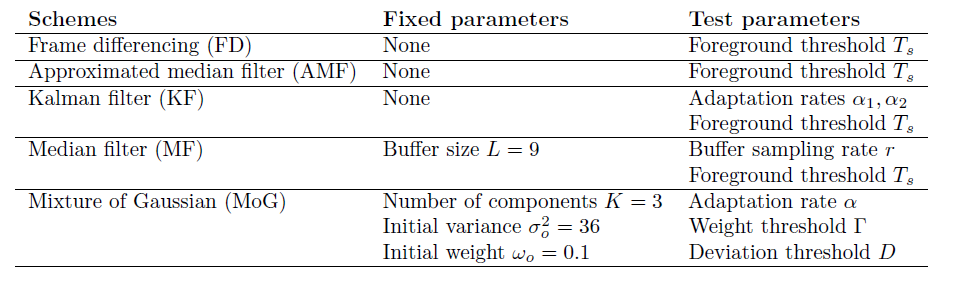
\includegraphics[scale=0.4]{./research/schemes} 
\end{center}
\caption{Background modelling schemes tested and their parameters \cite{Cheung2007}.}
\label{fig:background modelling schemes tested and their parameters}
\end{figure}

Cheung \cite{Cheung2007} selected four publicly-available urban traffic video sequences from the website maintained by KOGS/IAKS Universitaet Karlsruhey. A sample frame from each sequence is shown in Figure \ref{fig:sample frames from the four test sequences: Bright, Fog, Snow and Busy}.\\ 

\begin{figure}[h]
\begin{center}
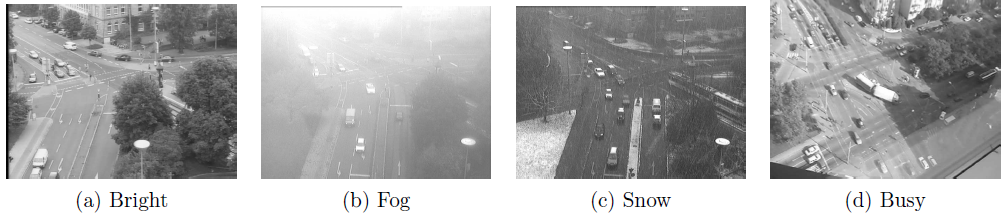
\includegraphics[scale=0.4]{./research/samples} 
\end{center}
\caption{Sample frames from the four test sequences: Bright, Fog, Snow and Busy. \cite{Cheung2007}.}
\label{fig:sample frames from the four test sequences: Bright, Fog, Snow and Busy}
\end{figure}

In Cheung's experiments \cite{Cheung2007} MoG achieved the best precision, MF was a very close second, followed by AMF and KF. FD was significantly worse than all the other schemes. Even though AMF performed worse than MoG and MF, it produced a good performance with an extremely simple implementation. The only drawback of AMF was that it adapts slowly toward a large change in background \cite{Cheung2007}. However this is not expected to be a problem for the tool kit as the should not be any large changes in the background of a doctor's office.\\

Visually, KF produced the worst foreground masks among all the schemes. Even with a large foreground threshold and slow adapting rates. as a result, it typically left a long trail after a moving object \cite{Cheung2007}. Slow updating may be an issue if the  person is required to move at all during the scan.\\

Such experiments suggest that, at this early stage, Adaptive Mean Filtering may be the way forward.\\